\documentclass[conference]{IEEEtran}
\usepackage{amsmath,amssymb}
\usepackage{graphicx}
\usepackage{booktabs}
\usepackage{siunitx}
\usepackage{cite}
% Generated by scripts/p2_make_paper.py from results/P2 (heldout seeds). Do not edit.
\newcommand{\pArray}{\ensuremath{8\times8}}
\newcommand{\pBinM}{5}
\newcommand{\pBlockedDb}{10}
\newcommand{\pBootN}{10{,}000}
\newcommand{\pBreakEven}{8--13}
\newcommand{\pBwA}{100}
\newcommand{\pBwB}{200}
\newcommand{\pBwC}{400}
\newcommand{\pCarrier}{28}
\newcommand{\pCi}{95}
\newcommand{\pClockBias}{50}
\newcommand{\pCloseEstFifteen}{+0.919}
\newcommand{\pCloseEstIdealFifteen}{+0.876}
\newcommand{\pCloseEstIdealRef}{+0.052}
\newcommand{\pCloseEstIdealThirty}{+0.121}
\newcommand{\pCloseEstIdealTwenty}{+0.732}
\newcommand{\pCloseEstIdealTwentyFive}{+0.373}
\newcommand{\pCloseEstRef}{+0.068}
\newcommand{\pCloseEstThirty}{+0.155}
\newcommand{\pCloseEstTwenty}{+0.656}
\newcommand{\pCloseEstTwentyFive}{+0.401}
\newcommand{\pClosePebLosFifteen}{+0.177}
\newcommand{\pClosePebLosRef}{+0.010$^\dagger$}
\newcommand{\pClosePebLosThirty}{+0.077}
\newcommand{\pClosePebLosTwenty}{+0.236}
\newcommand{\pClosePebLosTwentyFive}{+0.167}
\newcommand{\pClosePebMapFifteen}{-0.054$^\dagger$}
\newcommand{\pClosePebMapRef}{-0.025$^\dagger$}
\newcommand{\pClosePebMapThirty}{-0.018}
\newcommand{\pClosePebMapTwenty}{-0.037$^\dagger$}
\newcommand{\pClosePebMapTwentyFive}{-0.035$^\dagger$}
\newcommand{\pClosePerfFifteen}{-0.076$^\dagger$}
\newcommand{\pClosePerfRef}{-0.042}
\newcommand{\pClosePerfThirty}{-0.024}
\newcommand{\pClosePerfTwenty}{-0.064}
\newcommand{\pClosePerfTwentyFive}{-0.046$^\dagger$}
\newcommand{\pCloseWhiteFifteen}{+1.492}
\newcommand{\pCloseWhiteRef}{+0.098}
\newcommand{\pCloseWhiteThirty}{+0.191}
\newcommand{\pCloseWhiteTwenty}{+0.874}
\newcommand{\pCloseWhiteTwentyFive}{+0.399}
\newcommand{\pDecLosFourHundredAll}{74\%}
\newcommand{\pDecLosFourHundredBlk}{44\%}
\newcommand{\pDecLosFourHundredLos}{84\%}
\newcommand{\pDecLosHundredAll}{72\%}
\newcommand{\pDecLosHundredBlk}{43\%}
\newcommand{\pDecLosHundredLos}{81\%}
\newcommand{\pDecLosTwoHundredAll}{73\%}
\newcommand{\pDecLosTwoHundredBlk}{44\%}
\newcommand{\pDecLosTwoHundredLos}{82\%}
\newcommand{\pDecMapFourHundredAll}{98\%}
\newcommand{\pDecMapFourHundredBlk}{93\%}
\newcommand{\pDecMapFourHundredLos}{100\%}
\newcommand{\pDecMapHundredAll}{97\%}
\newcommand{\pDecMapHundredBlk}{87\%}
\newcommand{\pDecMapHundredLos}{100\%}
\newcommand{\pDecMapTwoHundredAll}{98\%}
\newcommand{\pDecMapTwoHundredBlk}{91\%}
\newcommand{\pDecMapTwoHundredLos}{100\%}
\newcommand{\pDecThr}{10}
\newcommand{\pEpoch}{0.1}
\newcommand{\pEstBlkAoa}{42}
\newcommand{\pEstBlkFourHundred}{36}
\newcommand{\pEstBlkHundred}{61}
\newcommand{\pEstBlkIdealHw}{33}
\newcommand{\pEstBlkKept}{13}
\newcommand{\pEstBlkSyncEpoch}{36}
\newcommand{\pEstBlkToa}{31}
\newcommand{\pEstBlkTwoHundred}{49}
\newcommand{\pEstBlkWorstHw}{48}
\newcommand{\pEstDecAoa}{45\%}
\newcommand{\pEstDecFourHundred}{47\%}
\newcommand{\pEstDecHundred}{28\%}
\newcommand{\pEstDecIdealHw}{51\%}
\newcommand{\pEstDecKept}{53\%}
\newcommand{\pEstDecSyncEpoch}{47\%}
\newcommand{\pEstDecToa}{45\%}
\newcommand{\pEstDecTwoHundred}{35\%}
\newcommand{\pEstDecWorstHw}{34\%}
\newcommand{\pEstLosAoa}{10}
\newcommand{\pEstLosFourHundred}{9}
\newcommand{\pEstLosHundred}{22}
\newcommand{\pEstLosIdealHw}{7}
\newcommand{\pEstLosKept}{8}
\newcommand{\pEstLosSyncEpoch}{9}
\newcommand{\pEstLosToa}{11}
\newcommand{\pEstLosTwoHundred}{18}
\newcommand{\pEstLosWorstHw}{16}
\newcommand{\pEstMedAoa}{13}
\newcommand{\pEstMedFourHundred}{12}
\newcommand{\pEstMedHundred}{26}
\newcommand{\pEstMedIdealHw}{10}
\newcommand{\pEstMedKept}{9}
\newcommand{\pEstMedSyncEpoch}{12}
\newcommand{\pEstMedToa}{13}
\newcommand{\pEstMedTwoHundred}{21}
\newcommand{\pEstMedWorstHw}{18}
\newcommand{\pEstPninetyAoa}{2.16}
\newcommand{\pEstPninetyFourHundred}{1.98}
\newcommand{\pEstPninetyHundred}{8.60}
\newcommand{\pEstPninetyIdealHw}{1.83}
\newcommand{\pEstPninetyKept}{1.02}
\newcommand{\pEstPninetySyncEpoch}{2.05}
\newcommand{\pEstPninetyToa}{1.90}
\newcommand{\pEstPninetyTwoHundred}{3.72}
\newcommand{\pEstPninetyWorstHw}{3.09}
\newcommand{\pEstRmseFourHundred}{7.2}
\newcommand{\pEstRmseHundred}{10.4}
\newcommand{\pEstRmseIdealHw}{6.3}
\newcommand{\pEstToPebAoa}{2}
\newcommand{\pEstToPebFourHundred}{2}
\newcommand{\pEstToPebHundred}{4}
\newcommand{\pEstToPebIdealHw}{35}
\newcommand{\pEstToPebKept}{2}
\newcommand{\pEstToPebSyncEpoch}{2}
\newcommand{\pEstToPebToa}{2}
\newcommand{\pEstToPebTwoHundred}{3}
\newcommand{\pEstToPebWorstHw}{1}
\newcommand{\pFdStep}{1}
\newcommand{\pGridSize}{144}
\newcommand{\pHwLosCalFive}{60\%}
\newcommand{\pHwLosIdeal}{92\%}
\newcommand{\pHwLosSyncThree}{92\%}
\newcommand{\pHwLosWorst}{45\%}
\newcommand{\pHwMapCalFive}{98\%}
\newcommand{\pHwMapIdeal}{99\%}
\newcommand{\pHwMapSyncThree}{99\%}
\newcommand{\pHwMapWorst}{97\%}
\newcommand{\pLimLosBase}{4.7}
\newcommand{\pLimLosBw}{0.97}
\newcommand{\pLimLosCal}{0.07}
\newcommand{\pLimLosSnr}{0.94}
\newcommand{\pLimLosSync}{0.72}
\newcommand{\pLimMapBase}{0.5}
\newcommand{\pLimMapBw}{0.71}
\newcommand{\pLimMapCal}{0.43}
\newcommand{\pLimMapSnr}{0.32}
\newcommand{\pLimMapSync}{0.44}
\newcommand{\pLitHigh}{0.8}
\newcommand{\pLitLow}{0.6}
\newcommand{\pMapToLosBlk}{0.09}
\newcommand{\pMapToLosP}{0.002}
\newcommand{\pMarginFifteen}{15}
\newcommand{\pMarginTwenty}{20}
\newcommand{\pMaxDepth}{2}
\newcommand{\pMaxPaths}{8}
\newcommand{\pNoiseFig}{7}
\newcommand{\pNscA}{792}
\newcommand{\pNscB}{1584}
\newcommand{\pNscC}{3168}
\newcommand{\pNumEl}{64}
\newcommand{\pNumRuns}{40}
\newcommand{\pNumSeeds}{10}
\newcommand{\pNumerology}{3}
\newcommand{\pPartOneRatio}{2.0}
\newcommand{\pPebLosFourHundredAll}{4.7}
\newcommand{\pPebLosFourHundredBlk}{12.5}
\newcommand{\pPebLosFourHundredLos}{4.1}
\newcommand{\pPebLosHundredAll}{4.8}
\newcommand{\pPebLosHundredBlk}{13.2}
\newcommand{\pPebLosHundredLos}{4.4}
\newcommand{\pPebLosTwoHundredAll}{4.7}
\newcommand{\pPebLosTwoHundredBlk}{12.6}
\newcommand{\pPebLosTwoHundredLos}{4.3}
\newcommand{\pPebMapFourHundredAll}{0.3}
\newcommand{\pPebMapFourHundredBlk}{1.1}
\newcommand{\pPebMapFourHundredLos}{0.3}
\newcommand{\pPebMapHundredAll}{0.7}
\newcommand{\pPebMapHundredBlk}{2.2}
\newcommand{\pPebMapHundredLos}{0.6}
\newcommand{\pPebMapTwoHundredAll}{0.5}
\newcommand{\pPebMapTwoHundredBlk}{1.5}
\newcommand{\pPebMapTwoHundredLos}{0.4}
\newcommand{\pPhiList}{0, 2 and 5}
\newcommand{\pPhiMain}{2}
\newcommand{\pPhiWorst}{5}
\newcommand{\pRatioLosA}{1.2}
\newcommand{\pRatioLosB}{3.0}
\newcommand{\pRatioMapA}{3.5}
\newcommand{\pRatioMapB}{4.3}
\newcommand{\pRatioPLosA}{0.004}
\newcommand{\pRatioPLosB}{0.002}
\newcommand{\pRatioPMapA}{0.002}
\newcommand{\pRatioPMapB}{0.002}
\newcommand{\pRatioPtwo}{2}
\newcommand{\pRatioThr}{5}
\newcommand{\pScs}{120}
\newcommand{\pSeedsDev}{1001--1010}
\newcommand{\pSeedsHeld}{2001--2010}
\newcommand{\pSeedsTune}{101--105}
\newcommand{\pSensRange}{40}
\newcommand{\pSyncList}{0, 0.3, 1 and 3}
\newcommand{\pSyncMain}{1}
\newcommand{\pSyncWorst}{3}
\newcommand{\pTxPower}{23}
\newcommand{\pUeHeight}{1.5}
\newcommand{\pVerdictFour}{mixed}
\newcommand{\pVerdictOneLos}{not supported}
\newcommand{\pVerdictOneMap}{not supported}
\newcommand{\pVerdictThree}{supported}
\newcommand{\pVerdictThreeKept}{supported}
\newcommand{\pVerdictTwo}{supported}
\newcommand{\pVerdictTwoKept}{not supported}

% DRAFT generated with the paper-2 pipeline (branch paper2). Every number is a
% macro from numbers2.tex (scripts/p2_make_paper.py, held-out seeds); author
% names and acknowledgements are left to the authors.

\begin{document}
\title{How Accurately Can mmWave Infrastructure Localize the User?\\ Bounds, Blockage and Hardware Limits}
\author{\IEEEauthorblockN{[Authors to be added]}}
\maketitle

\begin{abstract}
Blockage-aware proactive handover needs the user position to within about \pBreakEven\,cm, a requirement found in our companion study. We ask whether the two-O-RU \pCarrier\,GHz infrastructure that serves the user can deliver that accuracy from its own uplink sounding reference signals, at which bandwidth, and what happens during blockage. On a ray-traced street canyon with traffic-driven 3GPP blockage, we derive position error bounds that include inter-O-RU synchronization and array calibration errors as Bayesian priors, compare line-of-sight-only and map-aided (digital-twin) information, and build a practical beamspace/delay estimator with an EKF. On held-out seeds, decimeter bounds are not limited by bandwidth but by calibration: the line-of-sight-only bound reaches \pDecThr\,cm in \pDecLosFourHundredLos{} of the epochs with line of sight to both O-RUs at \pBwC\,MHz and still \pDecLosHundredLos{} at \pBwA\,MHz. A blocked line of sight that loses its geometric meaning raises the bound by a factor of \pRatioLosB, while map-aided reflections lower it to \pMapToLosBlk{} times the LoS-only value. The estimator reaches a median error of \pEstMedFourHundred\,cm, only \pPartOneRatio{} times the bound, but its heavy tails (90th percentile \pEstPninetyFourHundred\,m) make the paper-1 planner worse than 3GPP A5 at every margin.
\end{abstract}

\section{Introduction}
Millimeter-wave links are fragile under human and vehicle blockage~\cite{rappaport2013mmwave,maccartney2017blockage}. Integrated sensing and communication~\cite{liu2022isac} promises to anticipate blockage and hand the user over before the link breaks. Our companion study showed that such foresight beats the 3GPP A5 event only if the user position is known to about \pBreakEven\,cm. Street-canyon uplink positioning with several gNBs reports \pLitLow--\pLitHigh\,m RMSE~\cite{eswa2026srs}, and decimeter accuracy has so far been shown for target sensing rather than for the user. Classical bounds~\cite{shahmansoori2018position,abushaban2018bounds,shen2010fundamental} assume ideal hardware, under which the bound at the signal-to-noise ratios of a short street canyon is far below a centimeter and therefore uninformative.

We test four hypotheses, fixed before any held-out data was used: (P1) decimeter accuracy is theoretically possible only with wide bandwidth and line of sight (LoS) to both O-RUs; (P2) accuracy degrades sharply during blockage; (P3) map-aided use of reflected paths recovers part of that loss; (P4) a practical estimator stays well above the bound, and with its errors the paper-1 planner does not beat A5. Our contributions are (i) position error bounds with synchronization and calibration errors as Bayesian priors, two models of a blocked LoS and analytic image-method derivatives on the known facades; (ii) a practical estimator tuned on separate seeds; (iii) a closing experiment that feeds its positions into the frozen paper-1 planner; and (iv) a seed-level held-out evaluation of P1--P4.

\section{System Model}
\subsection{Scenario}
The scenario is that of the companion study: a ray-traced street canyon (Sionna RT~\cite{hoydis2023sionnart}, specular paths up to order \pMaxDepth, at most \pMaxPaths{} paths per link) at \pCarrier\,GHz with two O-RUs, each with a \pArray{} uniform planar array, and pedestrian user equipments (UEs) at height \pUeHeight\,m on the sidewalk. Cars, buses, trucks and pedestrians block every segment of every path according to 3GPP TR~38.901 blockage model~B~\cite{3gpp38901}. An O-RU is \emph{blocked} for a UE when its LoS loss is at least \pBlockedDb\,dB. Seeds: tuning \pSeedsTune, development \pSeedsDev, held-out \pSeedsHeld; each seed has \pNumRuns/\pNumSeeds{} runs (two mounts, two traffic densities), two UEs and one epoch every \pEpoch\,s.

\subsection{Signal model}
Each UE sends one uplink SRS symbol per epoch at \pTxPower\,dBm from a single antenna; each O-RU receives with noise figure \pNoiseFig\,dB. Numerology \pNumerology{} (\pScs\,kHz) with \pBwA, \pBwB{} and \pBwC\,MHz carriers uses \pNscA, \pNscB{} and \pNscC{} active subcarriers~\cite{3gpp38101_2}. At O-RU $c$, subcarrier $n$ and element $m$,
\begin{equation}
y_{c,n,m} = \textstyle\sum_p \beta_p\, e^{-j2\pi f_n(\tau_p+\delta_c+b)}\, e^{j\psi_{c,m}}\, s_m(\mathbf u_p) + w_{c,n,m},
\end{equation}
with complex path gains $\beta_p$ from the ray tracer and model~B, delays $\tau_p$, arrival directions $\mathbf u_p$, steering vector $s_m$, O-RU time offset $\delta_c\sim\mathcal N(0,\sigma_\mathrm{sync}^2)$ (\pSyncList\,ns, drawn once per run), per-element phase errors $\psi_{c,m}\sim\mathcal N(0,\sigma_\phi^2)$ (\pPhiList\,deg, fixed per O-RU and run) and UE clock bias $b$. Three timing cases are considered: synchronized ToA ($b$ known), TDoA ($b$ unknown) and AoA only. The main configuration uses TDoA, $\sigma_\mathrm{sync}=\pSyncMain$\,ns and $\sigma_\phi=\pPhiMain$\,deg.

\subsection{Blocked line of sight}
Model~B attenuates a blocked LoS but leaves its geometry intact. We therefore evaluate two variants: (a) \emph{kept}, where the attenuated LoS still carries exact delay and angle information (optimistic), and (b) \emph{biased}, where its delay and angles carry an unknown bias, i.e.\ its geometric information is removed. In the estimator, variant (b) is realized by letting the blocked LoS arrive via the shortest detour over or around its dominant blocker. Claims use (b).

\section{Position Error Bounds}
The Fisher information of the channel parameters follows from the Slepian--Bangs formula; the Gram matrix of the derivatives factorizes into frequency and antenna sums, so it is exact without synthesizing the channel. Complex gains are nuisance parameters and are eliminated by a Schur complement. The equivalent Fisher information in the horizontal position follows from the Jacobian of delays and angles and further Schur complements over the nuisance parameters~\cite{shen2010fundamental}: free path parameters (all reflected paths for LoS-only information, the blocked LoS in variant (b), all delays for AoA only), the clock bias, and the O-RU offsets and the $2\times\pNumEl$ element phases with their Gaussian priors (Bayesian information). For reflected paths, the derivatives are analytic by the image method on the known facades and ground; re-tracing at $\pm\pFdStep$\,cm validates them. The position error bound (PEB) is the square root of the trace of the inverse. An independent NumPy implementation (a single pseudo-inverse of the full information matrix) and a brute-force numeric Fisher matrix on a toy case verify the GPU code.

\section{Practical Estimator}
Per O-RU and epoch, a zero-padded 2-D DFT over the array finds the strongest beam; beamforming and a zero-padded, Hann-windowed delay transform give the delay of the dominant path, refined by parabolic interpolation, followed by an angle refinement at that delay. A peak-to-second-peak gate flags reflected dominant paths. Weighted least squares over the gated O-RUs, started from every single-O-RU angle fix (the planar array cannot distinguish the two sides of its plane), gives a fix and its covariance; a constant-velocity EKF tracks the UE. All thresholds, noise floors and the process noise ($\pGridSize$ grid points per bandwidth and timing case) were tuned on the tuning seeds only.

\section{Results (held-out seeds)}
All statistics use the seed as the unit: per-seed values over its runs, two-sided exact Wilcoxon signed-rank tests over the \pNumSeeds{} seeds and \pBootN-sample bootstrap intervals over seeds.

\subsection{Bounds}
Fig.~\ref{fig:bw} shows median bounds and estimator errors versus bandwidth. The LoS-only bound reaches \pDecThr\,cm in \pDecLosFourHundredLos{} of the epochs with LoS to both O-RUs at \pBwC\,MHz and \pDecLosHundredLos{} at \pBwA\,MHz, but only \pDecLosFourHundredBlk{} of the blocked epochs. The map-aided bound reaches it in \pDecMapFourHundredLos{} and \pDecMapFourHundredBlk{} of these epochs. P1 is therefore \textbf{\pVerdictOneLos}: bandwidth is not the limit. Relaxing one limit at a time at \pBwB\,MHz scales the median LoS-only bound (\pLimLosBase\,cm) by \pLimLosBw{} for twice the bandwidth, \pLimLosSnr{} for ten times the SNR, \pLimLosSync{} for perfect synchronization and \pLimLosCal{} for perfect calibration: calibration dominates. Without hardware errors the LoS-only bound reaches \pDecThr\,cm in \pHwLosIdeal{} of the epochs, with \pSyncWorst\,ns and \pPhiWorst\,deg errors in \pHwLosWorst; the map-aided bound stays at \pHwMapIdeal{} and \pHwMapWorst.

\begin{figure}[t]
\centering
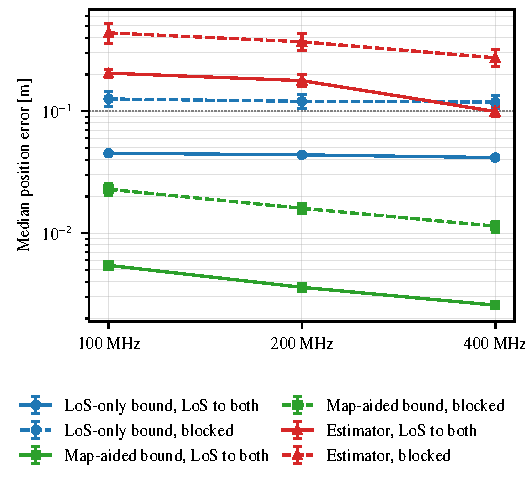
\includegraphics[width=\columnwidth]{figs/fig_p2_bw.pdf}
\caption{Median position error bound (LoS-only, map-aided) and median estimator error versus bandwidth, epochs with LoS to both O-RUs (solid) and with a blocked O-RU (dashed); main configuration; seed means with \pCi\,\% bootstrap intervals.}
\label{fig:bw}
\end{figure}

During blockage (variant (b)), the median LoS-only bound rises by a factor of \pRatioLosB{} ($p=\pRatioPLosB$): P2 is \textbf{\pVerdictTwo}. If the attenuated LoS kept its geometry (variant (a)), the factor would only be \pRatioLosA{} (P2 \pVerdictTwoKept). Map-aided information lowers the bound during blockage to \pMapToLosBlk{} times the LoS-only value ($p=\pMapToLosP$): P3 is \textbf{\pVerdictThree}. Fig.~\ref{fig:sidewalk} shows where along the sidewalk this happens.

\begin{figure}[t]
\centering
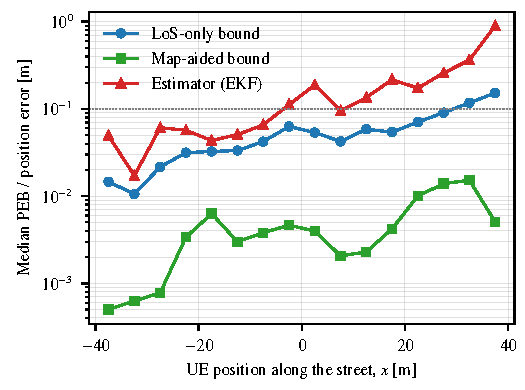
\includegraphics[width=\columnwidth]{figs/fig_p2_sidewalk.pdf}
\caption{Median bound and estimator error along the sidewalk (UE position, \pBinM\,m bins); main configuration.}
\label{fig:sidewalk}
\end{figure}

\subsection{Estimator}
At \pBwC\,MHz the estimator achieves a median error of \pEstMedFourHundred\,cm (\pEstLosFourHundred\,cm with LoS to both O-RUs, \pEstBlkFourHundred\,cm during blockage) and a 90th percentile of \pEstPninetyFourHundred\,m; at \pBwA\,MHz the median is \pEstMedHundred\,cm. Its median is within the \pLitLow--\pLitHigh\,m range of~\cite{eswa2026srs}, but its RMSE (\pEstRmseFourHundred\,m) is dominated by front/back mirror solutions and reflected dominant paths. The error is \pPartOneRatio{} times the LoS-only bound, i.e.\ not \emph{well} above it, because the same calibration error limits both (Fig.~\ref{fig:cdf}); without hardware errors the ratio rises to \pEstToPebIdealHw. A sync error drawn per epoch instead of once per run changes the median by less than a centimeter (\pEstMedSyncEpoch\,cm).

\begin{figure}[t]
\centering
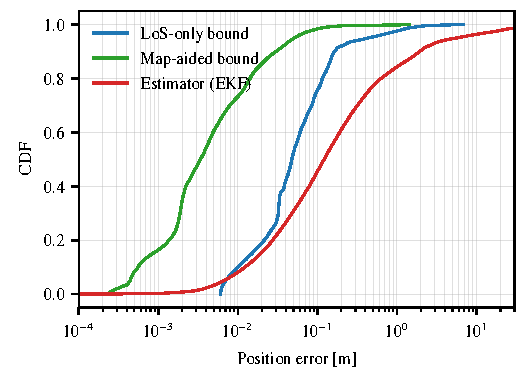
\includegraphics[width=\columnwidth]{figs/fig_p2_cdf.pdf}
\caption{CDF of the LoS-only and map-aided bounds and of the estimator error, main configuration; shaded: the paper-1 break-even range.}
\label{fig:cdf}
\end{figure}

\subsection{Closing experiment}
Fig.~\ref{fig:closing} feeds positions into the frozen paper-1 planner with perfect blocker tracks. With exact positions the planner is below A5 (\pClosePerfTwenty\,s/UE-min at \pMarginTwenty\,dB, \pClosePerfRef{} at the reference); with the map-aided bound-level error it stays close (\pClosePebMapTwenty, \pClosePebMapRef). Already the LoS-only bound-level error makes it worse (\pClosePebLosTwenty, \pClosePebLosRef), and the estimator's positions make it significantly worse than A5 at every margin from \pMarginFifteen\,dB (\pCloseEstFifteen, \pCloseEstTwenty, \pCloseEstTwentyFive, \pCloseEstThirty, \pCloseEstRef), even without hardware errors (\pCloseEstIdealTwenty{} at \pMarginTwenty\,dB). Daggers mark non-significant differences (pointwise, exploratory). Together with the estimator-to-bound ratio, P4 is \textbf{\pVerdictFour}.

\begin{figure}[t]
\centering
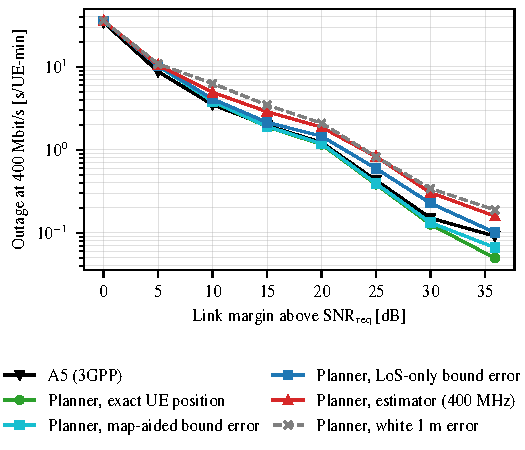
\includegraphics[width=\columnwidth]{figs/fig_p2_closing.pdf}
\caption{Outage at the service rate versus link margin: A5 and the paper-1 planner fed with UE positions of decreasing quality.}
\label{fig:closing}
\end{figure}

\section{Discussion and Limitations}
The infrastructure can localize the user to a decimeter in principle, but the binding limits are hardware calibration and the loss of LoS geometry during blockage, not bandwidth, and the practical bottleneck for proactive handover is the tail of the estimator error, not its median. The ray tracer is limited to specular paths of order \pMaxDepth{} with at most \pMaxPaths{} paths, which bounds what map-aided information can contribute; bodies are not traced as scatterers; the blocked-LoS detour is a modelling choice; the array is the companion study's \pArray{} planar array with its front/back ambiguity.

\section{Conclusion}
Decimeter user positioning from two \pCarrier\,GHz O-RUs is limited by array calibration and blockage rather than by bandwidth; map-aided reflections close the gap in theory, but a practical estimator's tail errors keep blockage-aware handover behind A5.

\bibliographystyle{IEEEtran}
\bibliography{refs2}
\end{document}
